\documentclass{article}

\usepackage{amsmath,amssymb}
\usepackage{geometry}
\usepackage{graphicx}

\geometry{a4paper, margin=2.5cm}

\begin{document}

% ============================================================
\section*{Direct Preference Optimization (DPO)}

\subsection*{First, a story}

Chapter 12's RLHF pipeline works but is heavy: first train a reward model, then run full PPO --- two stages, two models, plus all the instability of sampling-based training. An engineer looking at this pipeline asks a natural question: why must the information in preference data first be ``compressed'' into a reward model, only for RL to ``decompress'' it back into a policy?

\textbf{The naive approach}: supervised fine-tuning on the winning samples only (learn $y_w$, discard $y_l$). This degenerates into SFT, discarding the most valuable information in comparisons --- where the difference lies.

\textbf{This chapter's way}: note that KL-regularized reward maximization has a \textbf{closed-form optimum}; solve the reward back out through the optimal policy and substitute into the preference likelihood --- the reward model and PPO vanish together, leaving a purely supervised loss.

\textbf{The core question}: does skipping the reward-model component also skip the reward model's disease?

\[
\boxed{\mathcal{L}_{\mathrm{DPO}} = -\,\mathbb{E}_{(y_w, y_l)}\left[\log \sigma\!\left(\beta\log\frac{\pi_{\theta}(y_w)}{\pi_{\mathrm{ref}}(y_w)} - \beta\log\frac{\pi_{\theta}(y_l)}{\pi_{\mathrm{ref}}(y_l)}\right)\right]}
\]

\subsection*{Formalization}

Start from Chapter 12's objective: $\max_{\pi} \mathbb{E}_{y\sim\pi}[r(y)] - \beta\,\mathrm{KL}(\pi \| \pi_{\mathrm{ref}})$. Its optimum has closed form:

\[
\boxed{\pi^{*}(y) = \frac{1}{Z}\,\pi_{\mathrm{ref}}(y)\,\exp\!\left(\frac{r(y)}{\beta}\right)}
\]

Solving for the reward: $r(y) = \beta\log\frac{\pi^{*}(y)}{\pi_{\mathrm{ref}}(y)} + \beta\log Z$. Substituting into the Bradley--Terry likelihood $P(y_w \succ y_l)=\sigma(r(y_w)-r(y_l))$, the partition function $Z$ cancels in the difference, giving the DPO loss above.

\begin{itemize}
  \item $\pi_{\theta}$ --- the policy being optimized, which simultaneously plays the ``implicit reward model'';
  \item $\pi_{\mathrm{ref}}$ --- the frozen reference policy (the SFT model);
  \item $\beta$ --- the KL coefficient, of the same origin as Chapter 12's, now living inside the loss;
  \item $\hat{r}_{\theta}(y) = \beta\log\frac{\pi_{\theta}(y)}{\pi_{\mathrm{ref}}(y)}$ --- the implicit reward; training DPO fits it.
\end{itemize}

% ============================================================
\section*{Why the reward model can be skipped}

\subsection*{The policy is the reward model}

The BT likelihood depends only on reward differences, and the optimal policy corresponds one-to-one with the reward up to differences --- the policy's log-ratio \emph{is} the reward. So ``first learn the reward, then solve for the policy'' collapses into ``directly learn the policy'': DPO is an analytic shortcut to the same optimization problem, not a new objective.

The experiment compares the two roads on exactly the same toy task and the same 4000 preference pairs as Chapter 12: the RLHF pipeline (reward model + PPO, $\beta=0.5$) ends at a true score of about $+0.84$; DPO ($\beta=2.0$) crosses that line at about 1200 steps with a peak of about $+0.94\sim+1.05$ --- no reward model, no sampling-based training, comparable results (Figure~1).

\begin{figure}[!htbp]
  \centering
  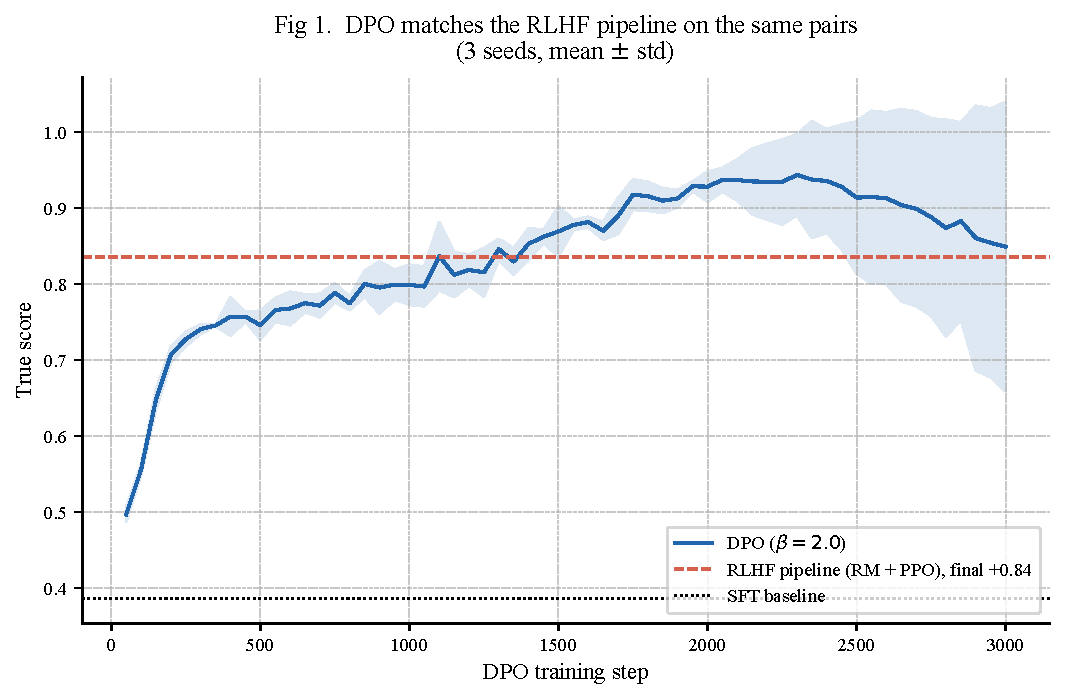
\includegraphics[width=0.88\textwidth]{fig1_dpo_vs_rlhf.pdf}
  \caption{On the same 4000 preference pairs, DPO ($\beta=2.0$) vs.\ Chapter 12's RLHF pipeline (reward model + PPO, $\beta=0.5$) (3 random seeds, shading $\pm 1\sigma$). DPO crosses the RLHF final level (dashed, $+0.84$) at about 1200 steps; after 2000 steps the mean slowly recedes and the cross-seed variance widens --- drift begins (see Figure~3).}
  \label{fig:dpo-vs-rlhf}
\end{figure}

% ============================================================
\section*{Core mechanisms}

\subsection*{Mechanism 1: the implicit reward, the same disease}

DPO training fits the implicit reward $\hat{r}_{\theta}=\beta\log(\pi_{\theta}/\pi_{\mathrm{ref}})$, which obeys the same law as Chapter 12's explicit reward model: \textbf{trustworthy only within the preference data's coverage}. Grouping the trained policy's implicit reward by emphasis-token count (Figure~2): inside the coverage it rises with the true score; outside, the true score peaks and collapses while the implicit reward keeps rising monotonically --- the same extrapolation curve as Chapter 12's Figure~1 (right). Skipping the component does not skip the fact that the reward comes from finitely covered data.

\begin{figure}[!htbp]
  \centering
  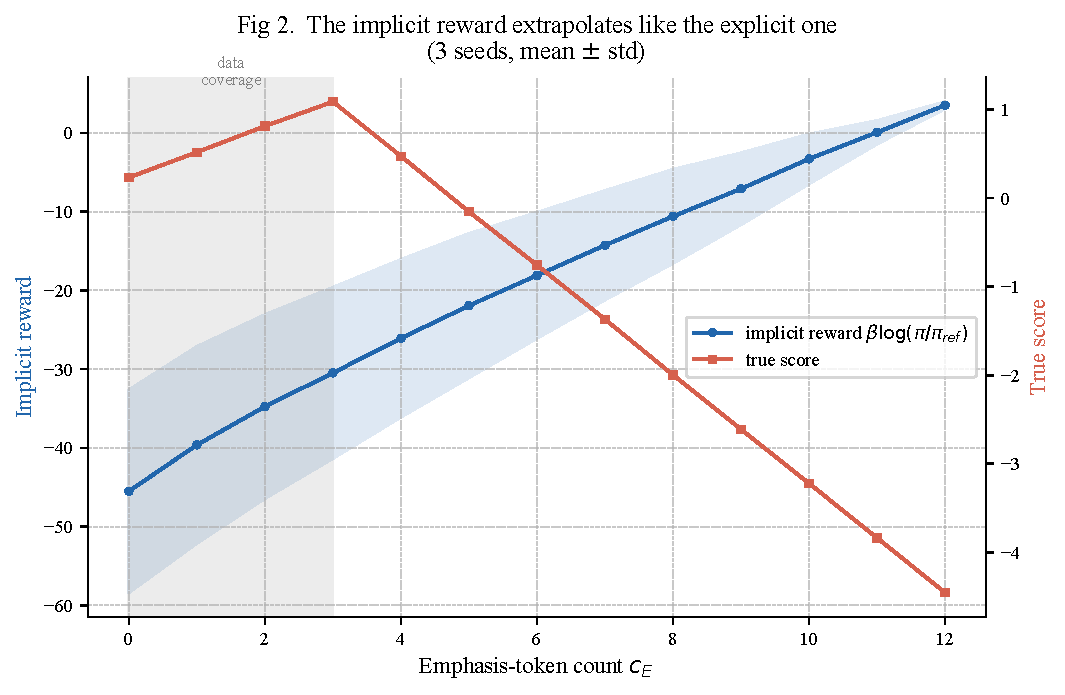
\includegraphics[width=0.88\textwidth]{fig2_implicit_reward.pdf}
  \caption{The implicit reward $\beta\log(\pi/\pi_{\mathrm{ref}})$ of the trained policy ($\beta=0.1$, the collapsing group of Figure~3), grouped by emphasis-token count $c_E$ (3 random seeds, shading $\pm 1\sigma$). Within the preference-data coverage (gray, $c_E\le 3$) the implicit reward tracks the true score; outside, the true score collapses while the implicit reward keeps rising monotonically --- isomorphic to the explicit reward model's extrapolation.}
  \label{fig:dpo-implicit}
\end{figure}

\subsection*{Mechanism 2: the soft anchor --- $\beta$ and training length jointly set the drift}

Chapter 12's KL penalty is an explicit term in the objective; DPO's $\beta$ hides inside the loss, a \textbf{soft anchor}. The gradient weight is $\sigma(-\beta\cdot\mathrm{margin})$: the larger the margin, the smaller the weight --- but as long as the loss is unsaturated, the $\log(\pi_{\theta}/\pi_{\mathrm{ref}})$ gap keeps being amplified. Smaller $\beta$ saturates more slowly and amplifies faster.

The key experimental fact (Figure~3): DPO \textbf{never samples its own generations}, yet token-level generalization still pushes the generation distribution out of the coverage --- $\beta=0.1$ collapses within a few hundred steps (final about $-3.8$); $\beta=0.5$ collapses more slowly but equally (about $-4.1$); $\beta=2.0$ stays near $+0.85$, with widening cross-seed variance late in training --- the drift has begun. Training length is therefore DPO's \textbf{hidden hyperparameter}: early stopping is not optional but part of the anchor.

\begin{figure}[!htbp]
  \centering
  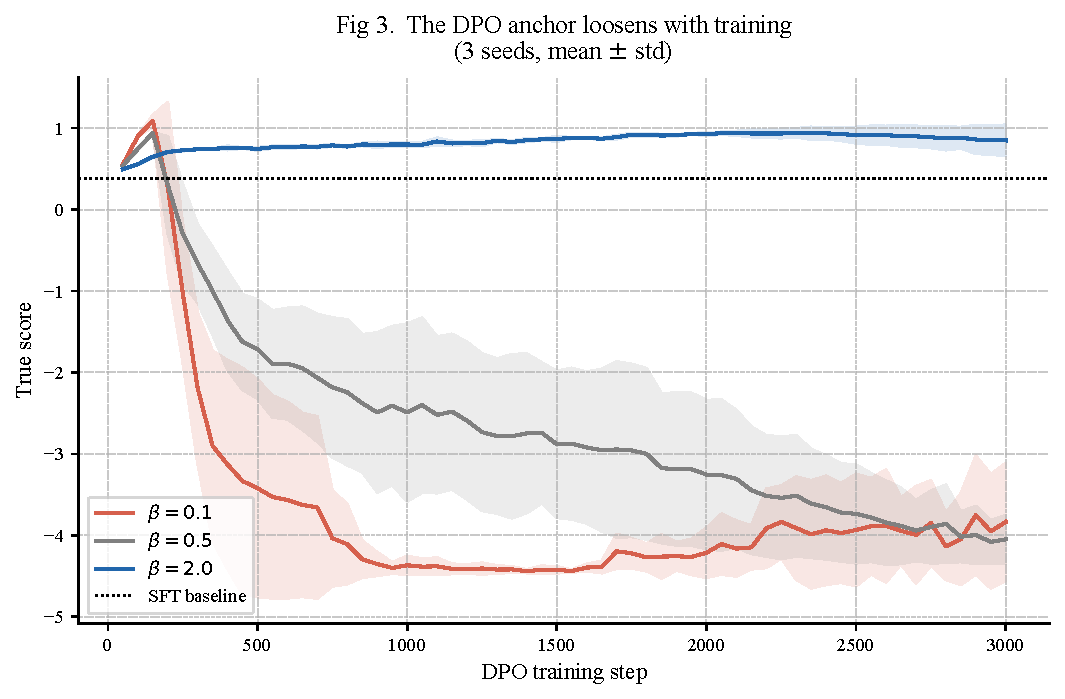
\includegraphics[width=0.88\textwidth]{fig3_beta_anchor.pdf}
  \caption{$\beta$ sweep (3 random seeds, shading $\pm 1\sigma$; dash-dotted line, the SFT baseline $+0.39$). $\beta=0.1$ briefly spikes then collapses within a few hundred steps (final about $-3.8$); $\beta=0.5$ collapses more slowly but equally (about $-4.1$); $\beta=2.0$ stays near $+0.85$ with late-training variance widening --- DPO's anchor loosens with training.}
  \label{fig:dpo-anchor}
\end{figure}

\subsection*{Mechanism 3: the gradient shape --- built-in hard-example weighting}

Differentiating the DPO loss: the scalar weight in front of the gradient is $\sigma(-\beta\cdot\mathrm{margin})$ --- pairs currently misclassified (negative margin) get weight near 1; pairs already correctly ranked with large margin get weight near 0. DPO naturally concentrates learning pressure on comparisons ``the policy cannot yet distinguish'' --- one source of its training stability.

% ============================================================
\section*{The full pipeline}

\subsection*{Three steps}

\begin{enumerate}
  \item \textbf{SFT}: obtain the reference policy $\pi_{\mathrm{ref}}$; freeze it;
  \item \textbf{Preference collection}: sample pairs from $\pi_{\mathrm{ref}}$ and label them (as in RLHF);
  \item \textbf{Direct optimization}: initialize $\pi_{\theta}\leftarrow\pi_{\mathrm{ref}}$ and minimize $\mathcal{L}_{\mathrm{DPO}}$; sequence log-probabilities sum over tokens, and the margin is the difference of ``policy minus reference'' differences; stop by generation quality or validation KL.
\end{enumerate}

% ============================================================
\section*{DPO vs RLHF}

\begin{itemize}
  \item \textbf{Components}: RLHF needs a reward model + PPO (sampling, advantage estimation, ratio clipping); DPO has a single supervised loss;
  \item \textbf{Failure mode}: the same disease (optimistic extrapolation beyond the coverage) with different onsets --- PPO \textbf{actively searches} for the fork by sampling, DPO \textbf{passively drifts} out by generalization; the former collapses fast (within 60 iterations in Chapter 12), the latter at a pace set by $\beta$ and training length;
  \item \textbf{The nature of the anchor}: RLHF's KL is an explicit penalty in the objective; DPO's $\beta$ is a soft anchor inside the loss --- soft anchors loosen with training and must be paired with early stopping.
\end{itemize}

% ============================================================
\section*{Where this chapter sits in the RL landscape}

\begin{enumerate}
  \item Upstream: RLHF (Chapter 12) supplies the objective --- KL-regularized reward maximization from preferences;
  \item \underline{Direct Preference Optimization} (this chapter: an analytic shortcut to the same objective --- the policy is the reward model);
  \item Downstream: GRPO and verifiable rewards (RLVR) --- when task correctness is decidable by rule, verifiable rewards replace learned ones, and ``the reward gets hacked'' becomes impossible by construction.
\end{enumerate}

The takeaway: \textbf{DPO changes the implementation path, not the structure of the problem --- the preference data's coverage remains the optimizable boundary; only this time, crossing it relies not on the sampler's search but on the network's own generalization}. The next chapter swaps out the source of the reward.

\subsection*{References}

\begin{enumerate}
  \item Rafailov et al.\ (2023). Direct Preference Optimization: Your Language Model is Secretly a Reward Model. \textit{NeurIPS}.
  \item Azar et al.\ (2024). A General Theoretical Paradigm to Understand Learning from Human Preferences (IPO). \textit{AISTATS}.
  \item Tunstall et al.\ (2023). Zephyr: Direct Distillation of LM Alignment. \textit{arXiv:2310.16944}.
  \item Ouyang et al.\ (2022). Training Language Models to Follow Instructions with Human Feedback. \textit{NeurIPS}.
\end{enumerate}

\end{document}
